\documentclass[12pt,a4paper]{article}

% Margins.
\setlength{\oddsidemargin}{0in}
\setlength{\evensidemargin}{0in}
\setlength{\headheight}{12pt}
\setlength{\headsep}{42pt}
\setlength{\topmargin}{-54pt}
\setlength{\textwidth}{6.5in}
\setlength{\textheight}{10in}

\usepackage{amsmath}
\usepackage{float}
\usepackage{graphicx}
\usepackage[hyphens]{url}
\usepackage{hyperref}	% Clickable links to figures, references and urls.
\usepackage{datetime}
\usepackage{longtable}
\usepackage{subfigure}

% Links direct to top of figures.
\usepackage[all]{hypcap}

% Drawing.
\usepackage{pgf}
\usepackage{tikz}

% Listings for formatting code.
\usepackage{listings}
\usepackage{textcomp}
% General options.+++
\lstset{breaklines=true, basicstyle=\small\ttfamily, tabsize=4, numbers=left, stepnumber=1, frame=single, showstringspaces=false, upquote=true}
% C++ specific high-lighting. Comments are 50/50 shades of green/black and strings coloured with 60/40 red/black mixture.
\lstset{language=[ISO]C++, commentstyle=\color{green!50!black}, keywordstyle=\color{blue}, stringstyle=\color{red!60!black}}

%opening
\title{\vspace{-3cm}Physics for Engineers\\Class 27\\Electric Potential}
\author{Attique Dawood}
\date{October 25, 2013\\[0.2cm] Last Modified: \today, \currenttime}
\begin{document}
\maketitle
\section{Announcements}
\begin{itemize}
\item None.
\end{itemize}
\section{Shielding}
There are two kinds of shielding.
\begin{enumerate}
\item When you want to isolate some sensitive equipment from outside interference you enclose that equipment in a metallic casing. The device may emit radiation but it won't be affected by any field outside the metallic cage (Faraday's cage). Example is a +q charge placed inside a (neutral) metallic shell.
\item When you want to eliminate electromagnetic radiation: If a positive charge +q is covered with metallic shell having -q charge then no field will exist outside the shell. In this kind of shielding +q charge will not be affected any field outside the shell. Also, there won't be any field outside the shell. Example is coaxial cable, inner conductor carries +ve current and outer conductor carries -ve current and there is not field outside the wire.
\end{enumerate}
\section{Electric Potential}
Suppose an electric field exists in some region. We take a charge $q$ and move it around. We know that a force $\textbf{F}=q\textbf{E}$ will act on the charge. If we want to move the charge from point A to point B then the total amount of work that must be done by us (to overcome the field) is given by
\begin{equation}
W=\Delta U=U_B-U_A=-q\int\limits_{a}^{b} \textbf{E}\cdot d\textbf{\textit{l}}.
\end{equation}
Here $\Delta U$ is the energy difference between points A and B as we move a charge $q$. \textbf{Electric field stores energy} and a detailed discussion will have to be deferred for later. From here we define another quantity called electric potential (V).
\begin{equation}
V=\dfrac{U}{q}.
\end{equation}
Or
\begin{equation}
\Delta V=\dfrac{\Delta U}{q}.
\end{equation}
To calculate potential difference between two points, A and B, in electric field \textbf{E}
\begin{equation}
\Delta V=V_{AB}=V_B-V_A=-\int\limits_{a}^{b} \textbf{E}\cdot d\textbf{\textit{l}}.
\end{equation}
Notice, that just as electric field was a fundamental quantity where we can find force on \textit{any} charge $q$ by simply multiplying it with \textbf{E}, electric potential is also a fundamental quantity where we can find the energy difference between two points, A and B, by simply multiplying $q$ with $V_{AB}$. $W=\Delta U=U_{AB}=qV_{AB}$ gives the amount of work that must be done in moving \textit{any} charge $q$ from A to B in electric field.
\section{Absolute Potential}
Absolute potential at some point B is the potential difference at B with respect to infinity. Or, it is the potential difference between A and B when point A or initial point is at infinity. Absolute potential is a useful standard reference point that can be used to define a potential scalar field. Remember, electric potential is a scalar quantity.
\begin{equation}
V_B=-\int\limits_{\infty}^{b} \textbf{E}\cdot d\textbf{\textit{l}}.
\end{equation}
Note, when referring to electric potential as `potential at some point' or simply `potential' then this usually means absolute electric potential at that point.
\section{Exercises}
\noindent\textbf{Question 1:} Electric field in a region is $\textbf{E}=\dfrac{1}{4\pi\epsilon_0x^2}\hat x$ V/m. Find absolute potential $V_b$ at a point $x=b$.\\[0.2cm]
\noindent\textbf{Question 2:} Find absolute potential field of a point charge.
%\begin{itemize}
%\item[a.] Electric field of a point charge.
%\item[b.] Electric field of an infinite line charge placed along $z$--axis.
%\end{itemize}
%%\begin{figure}[H]
%\centering
%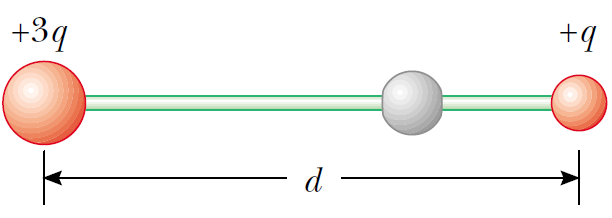
\includegraphics[scale=0.45]{FigureP23-10.png}
%\caption{Equilibrium of charge.}
%\label{Equilibrium}
%\end{figure}
%\nocite{*}
%\bibliographystyle{plain}
%\bibliography{PhysicsRef}
\end{document}
